\documentclass{article}
\usepackage{iclr2025_conference,times}

\usepackage{graphicx}
\usepackage{hyperref}
\usepackage{url}

\iclrfinalcopy
\pagestyle{empty}

\title{A Market-Rule-Informed Neural Network for Efficient Imbalance Electricity Price Forecasting}
\author{\textbf{Runyao Yu$^{1,2}$, Julia Lin$^2$, Derek W. Bunn$^3$, Jochen Stiasny$^1$, Wentao Wang$^4$}\\\textbf{Yujie Chen$^5$, Tara Esterl$^2$, Peter Palensky$^1$, Jochen L. Cremer$^{1,2}$}\\[0.25em]\footnotesize $^1$Delft University of Technology, $^2$Austrian Institute of Technology, $^3$London Business School\\\footnotesize $^4$University of Technology Sydney, $^5$The Chinese University of Hong Kong (Shenzhen)}

\makeatletter
\newcommand{\DeepPriorLogoRow}{%
  \AddToShipoutPictureFG*{%
    \AtPageUpperLeft{%
      \put(\LenToUnit{8.10in},\LenToUnit{-1.23in}){%
        \makebox[0pt][r]{
\includegraphics[width=0.825in,keepaspectratio]{deepprior-logo.png}}%
      }%
    }%
  }%
}

\newcommand{\DeepPriorTitleRow}{%
  \noindent\makebox[\textwidth][c]{%
    \begin{minipage}[c]{\textwidth}
      \centering\LARGE\bfseries \@title
    \end{minipage}%
  }\par
}

\newcommand{\DeepPriorAuthors}{%
  \begin{center}
    \begin{tabular}{c}\@author\end{tabular}
  \end{center}
}

\newcommand{\DeepPriorAbstract}[1]{%
  \begin{center}{\large\sc Abstract}\end{center}\vspace{-0.35em}%
  \begin{quote}#1\end{quote}%
}

\newcommand{\DeepPriorFigure}{%
  \noindent\makebox[\textwidth][c]{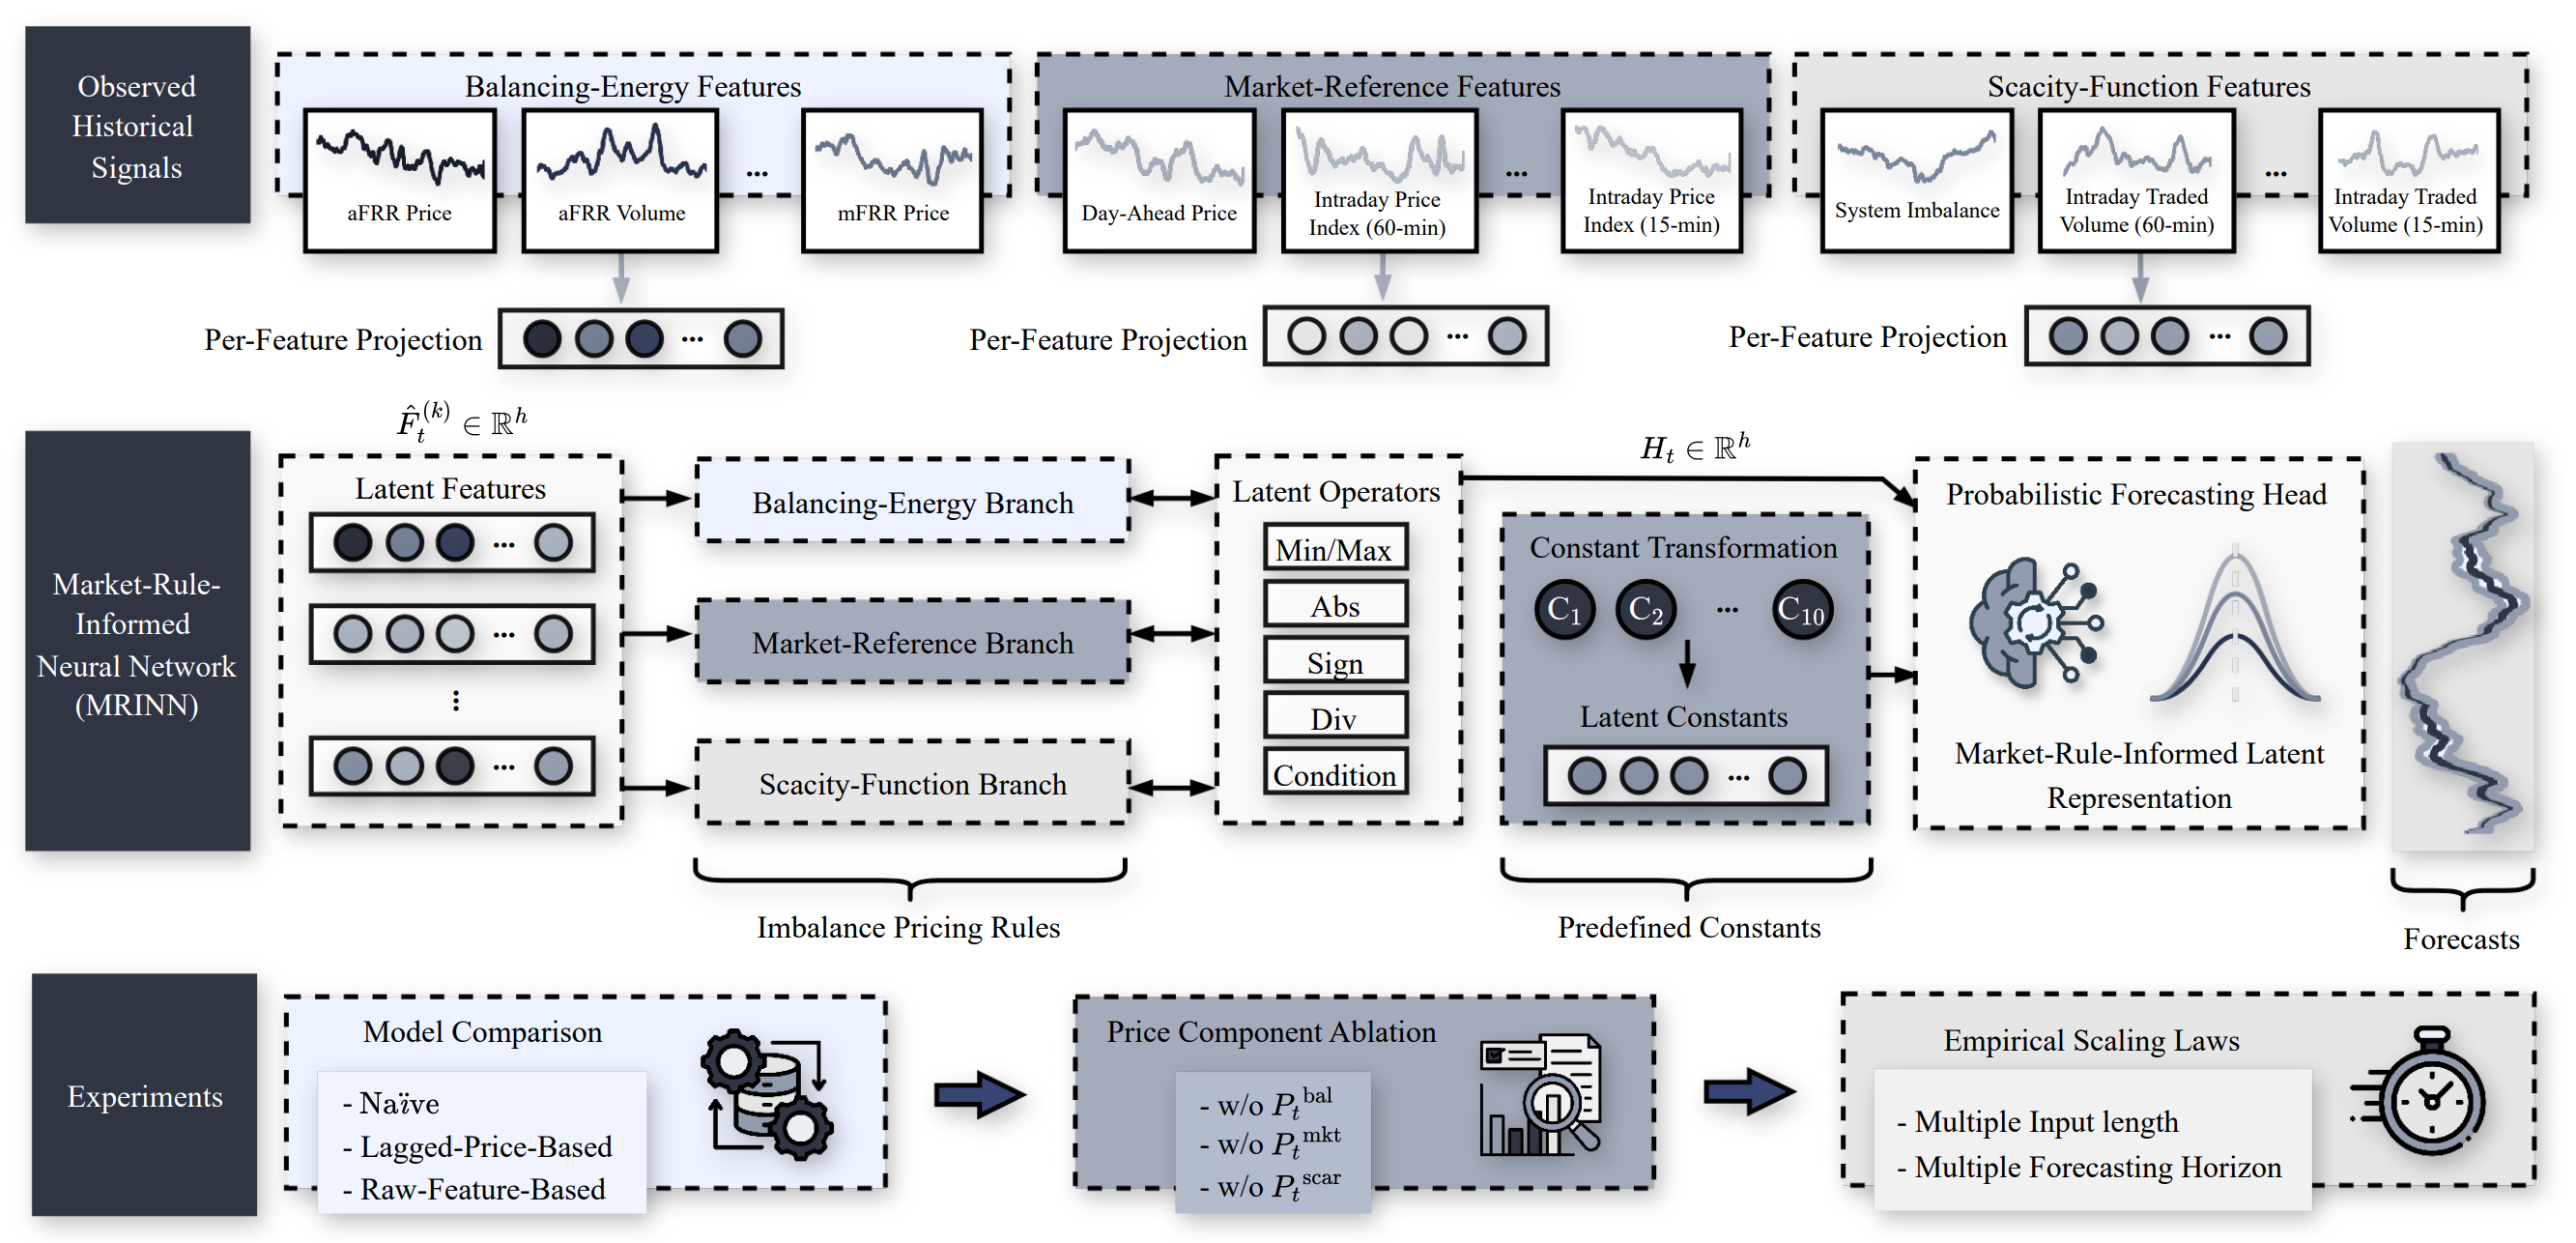
\includegraphics[width=\textwidth,keepaspectratio]{figure.png}}\par
  \vspace{2pt}%
  \noindent\makebox[\textwidth][c]{{\small Figure~1: Structure of MRINN and the corresponding experimental analysis.}}%
}

\makeatother
\begin{document}
\fancyhf{}
\renewcommand{\headrulewidth}{0pt}
\thispagestyle{empty}
\makeatletter
\DeepPriorLogoRow
\noindent\begin{minipage}[t][\dimexpr\textheight-\baselineskip\relax][s]{\textwidth}
\vspace*{0.50in}
\vfill
\DeepPriorTitleRow
\vfill
\DeepPriorAuthors
\vfill
\DeepPriorAbstract{Accurate and efficient imbalance electricity price forecasting is critical for industrial energy trading systems, especially as battery assets and automated bidding pipelines increasingly participate in balancing markets. However, real-time forecasting is complicated by nonlinear market-rule-based price formation, heterogeneous input signals, and incomplete data availability caused by communication delays, publication lags, and measurement outages. This paper proposes a market-rule-informed neural forecasting framework that embeds imbalance price formation rules into the latent space of an expressive neural network. The proposed framework preserves raw signal information while exploiting transparent market-rule priors. We further analyze operational robustness by removing price-component information and characterize how forecasting performance scales with input length and forecasting horizon. Experimental results show that the proposed model achieves competitive forecasting performance with substantially fewer trainable parameters and shorter training time than generic deep learning baselines, demonstrating that market-rule priors and expressive neural networks should be jointly used for accurate and computationally sustainable forecasting in industrial energy trading applications.}
\vfill
\DeepPriorFigure
\end{minipage}
\makeatother
\end{document}
